% !TEX root = ../thesis-index.tex


\chapter{Batch normalization without gradient explosion}\label{ch:bn_grad}

% Wrote an alternative introduction
% \section{Introduction}
% \label{grad:sec:introduction}
\blfootnote{Code is available at: \url{https://github.com/alexandrumeterez/bngrad}}
%\paragraph{Training deep neural networks issues.}
What if we could train even deeper neural networks? Increasing depth empowers neural networks, by turning them into powerful data processing machines. For example, increasing depth allows large language models (LLMs) to capture longer structural dependencies~\citep{devlin2018bert,liu2019roberta,brown2020language,goyal2021larger,raffel2020exploring}. Also, sufficiently deep convolutional networks can outperform humans in image classification~\citep{liu2022convnet,woo2023convnext,wu2021cvt}. Nevertheless, increasing depth imposes an inevitable computational challenge: deeper networks are harder to optimize. In fact, standard optimization methods exhibit a slower convergence when training deep neural networks. Hence, computation has become a barrier in deep learning, demanding extensive research and engineering. 

A critical problem is that deeper networks suffer from the omnipresent issue of rank collapse at initialization: the outputs become collinear for different inputs as the network grows in depth~\citep{saxe2013exact}. Rank collapse is not only present in MLPs and convolutional networks~\citep{feng2022rank,saxe2013exact,daneshmand2020batch}, but also in transformer architectures~\citep{dong2021attention, noci2022signal}. This issue significantly contributes to the training slowdown of deep neural networks. Hence, it has become the focus of theoretical and experimental studies~\citep{saxe2013exact,feng2022rank,daneshmand2021batch,noci2022signal}.  

One of the most successful methods to avoid rank collapse is Batch Normalization (BN)~\citep{ioffe2015batch}, as proven in a number of theoretical studies ~\citep{yang2018a, daneshmand2020batch, daneshmand2021batch}. Normalization imposes a particular bias across the layers of neural networks~\citep{joudaki2023impact}. More precisely, the representations of a batch of inputs become more orthogonal after each normalization~\citep{joudaki2023impact}. This orthogonalization effect precisely avoids the rank collapse of deep neural networks at initialization~\citep{yang2018a,joudaki2023impact,daneshmand2021batch,joudaki2023bridging}. 

While batch normalization effectively avoids rank collapse, it causes numerical issues. The existing literature proves that batch normalization layers cause exploding gradients in MLPs in an activation-independent manner~\cite{yang2018a}. Gradient explosion limits increasing depth by causing numerical issues during backpropagation. For networks without batch normalization, there are effective approaches to avoid gradient explosion and vanishing, such as tuning the variance of the random weights based on the activation and the network width~\citep{he2015delving,glorot2010understanding}. However, such methods cannot avoid gradient explosion in the presence of batch normalization~\cite{yang2018a}. Thus, the following important question remains unanswered:  
\begin{center} \emph{Is there any network with batch normalization without gradient explosion and rank collapse issues?}\end{center}

\paragraph{Contributions.}
We answer the above question affirmatively by giving a specific MLP construction initialized with orthogonal random weight matrices, rather than Gaussian. To show that the MLP still has optimal signal propagation, we prove that the MLP output embeddings become isometric (\eqref{grad:eq:iso_gap}), implying the output representations becomes more orthogonal with depth. For a batch of linearly independent inputs, we prove
\begin{align}\label{grad:eq:iso_gap_decay}
    \E\big[\text{isometry gap}\big] = \mathcal{O}\left( e^{-\text{depth}/C}\right),
\end{align}
where $C$ is a constant depending only on the network width and input and the expectation is taken over the random weight matrices. Thus, for sufficiently deep networks, the representations rapidly approach an orthogonal matrix. While \citet{daneshmand2021batch} prove that the outputs converge to within an $\mathcal{O}(\text{width}^{-1/2})$-ball close to orthogonality, we prove that the output representations become perfectly orthogonal in the infinite depth limit. This perfect orthogonalization turns out to be key in proving our result about avoiding gradient explosion. In fact, for MLPs initialized with Gaussian weights and BN, \citet[Theorem 3.9]{yang2018a} prove that the gradients explode at an exponential rate in depth. In a striking contrast, we prove that gradients of an MLP with BN and orthogonal weights remain bounded as
\begin{align}\label{grad:eq:grad_norm_bounded}
    \E \big[
\log\left(\text{gradient norm for each layer}\right)\big] = \mathcal{O}\left( \text{width}^5\right).
\end{align}
Thus, the gradient is bounded by a constant that only depends on the network width where the expectation is taken over the random weight matrices. It is worth noting that both isometry and log-norm gradient bounds are derived \emph{non-asymptotically}. Thus, in contrast to the previously studied mean field or infinite width regime, our theoretical results hold in practical settings where the width is finite. 

The limitation of our theory is that it holds for a simplification in the BN module and linear activations. However, our results provide guidelines to avoid gradient explosion in MLPs with non-linear activations. We experimentally show that it is possible to avoid gradient explosion for certain non-linear activations with orthogonal random weights together with ``activation shaping''~\cite{martens2021rapid}. Finally, we experimentally demonstrate that avoiding gradient explosion stabilizes the training of deep MLPs with BN. 

\section{Related work}
\label{grad:sec:related_work}
\paragraph{The challenge of depth in learning.} Large depth poses challenges for the optimization of neural networks, which becomes slower by increasing the number of layers. This depth related slowdown is mainly attributed to: (i) gradient vanishing/explosion, and (ii) the rank collapse of hidden representations. (i) Gradient vanishing and explosion is a classic problem in neural networks ~\citep{hochreiter1998vanishing}. For some neural architectures, this issue can be effectively solved. For example, \citet{he2015delving} propose a particular initialization scheme that avoids gradient vanishing/explosion for neural networks with rectifier non-linearities while  \citet{glorot2010understanding} study the effect of initialization on sigmoidal activations. However, such initializations cannot avoid gradient explosion for networks with batch normalization~\citep{yang2018a,lubana2021beyond}. (ii) \citet{saxe2013exact} demonstrate that outputs become independent from inputs with growing depth, which is called the rank collapse issue~\citep{daneshmand2020batch,dong2021attention}. Various techniques have been developed to avoid rank collapse such as batch normalization~\cite{ioffe2015batch}, residual connections~\cite{he2016res}, and self-normalizing activations~\cite{klambauer2017self}. A related line of work has shown how signal propagation can be achieved without batch normalization in feed-forward networks ~\citep{burkholz2019initialization} and ResNets~\citep{brock2021characterizing}.
Other works on CNNs~\cite{blumenfeld2020beyond} have shown that symmetry breaking is a vital element for achieving signal propagation with stable gradients in deep models. 
Here, we focus on batch normalization since our primary goal is to avoid the systemic issue of gradient explosion for batch normalization.

\paragraph{Initialization with orthogonal matrices.}
\citet{saxe2013exact} propose initializing the weights with random orthogonal matrices for linear networks without normalization layers. Orthogonal matrices avoid the rank collapse issue in linear networks, thereby enabling a depth-independent training convergence. \citet{pennington2017resurrecting} show that MLPs with sigmoidal activations achieve dynamical isometry when initialized with orthogonal weights. Similar benefits have been achieved by initializing CNNs with orthogonal or almost orthogonal kernels~\citep{xiao2018dynamical,mishkin2015all}, and by initializing RNN transition matrices with elements from the orthogonal and unitary ensembles ~\citep{arjovsky2016unitary,le2015simple,henaff2016recurrent}. Similarly, we use orthogonal random matrices to avoid gradient explosion. What sets our study apart from this literature is that our focus is on batch normalization and the issue of gradient explosion.

\paragraph{Networks with linear activation functions.}
Due to its analytical simplicity, the identity function has been widely used in theoretical studies for neural networks. Studies on identity activations date back to at least two decades. \citet{fukumizu1998effect} studies batch gradient descent in linear neural networks and its effect on overfitting and generalization. \citet{baldi1995learning} provide an overview over various theoretical manuscripts studying linear neural networks. Despite linearity, as \citet{saxe2013exact, saxe2013learning} observe, the gradient dynamics in a linear MLP are highly nonlinear. In a line of work,  \citet{saxe2013learning,saxe2013exact, saxe2019mathematical} study the training dynamics of deep neural networks with identity activations and introduce the notion of dynamical isometry. \citet{baldi1989neural} and \citet{yun2017global} study the mean squared error optimization landscape in linear MLPs. More recently, the optimum convergence rate of gradient descent in deep linear neural networks has been studied by \citet{arora2018convergence} and \citet{shamir2019exponential}. \citet{du2019width} prove that under certain conditions on the model width and input degeneracy, linear MLPs with Xavier initialized weights~\citep{glorot2010understanding} converge linearly to the global optimum. Akin to these studies, we also analyze networks with linear activations. However, batch normalization is a non-linear function, hence the network we study in this chapter is a highly non-linear function of its inputs.

\paragraph{Mean field theory for random neural networks.} 
The existing analyses for random networks often rely on mean field regimes where the network width tends to infinity~\citep{pennington2017resurrecting,yang2018a,li2022neural,pennington2017nonlinear}. However, there is a discrepancy between mean field regimes and the practical regime of finite width. While some analyses attempt to bridge this gap~\citep{joudaki2023bridging,daneshmand2021batch}, their results rely on technical assumptions that are hard to validate. In contrast, our non-asymptotic results hold for standard neural networks used in practice. Namely, our main assumption for avoiding rank collapse and gradient explosion is that samples in the input batch are not linearly dependent, which we will show is necessary. To go beyond mean field regimes, we leverage recent theoretical advancements in Weingarten calculus~\citep{weingarten1978asymptotic, collins2003moments, banica2011polynomial, collins2006integration, collins2022weingarten}.


\paragraph{Mean field theory for random neural networks.}\label{grad:sec:supp_rel_work}
The existing analyses for random networks often rely on mean field regimes where the network width tends to infinity~\citep{pennington2017resurrecting,yang2018a,li2022neural,pennington2017nonlinear}. However, there is a discrepancy between mean field regimes and the practical regime of finite width. While some analyses attempt to bridge this gap~\citep{joudaki2023bridging,daneshmand2021batch}, their results rely on technical assumptions that are hard to validate. In contrast, our non-asymptotic results hold for standard neural networks used in practice. Namely, our main assumption for avoiding rank collapse and gradient explosion is that samples in the input batch are not linearly dependent, which we will show is necessary. To go beyond mean field regimes, we leverage recent theoretical advancements in Weingarten calculus~\citep{weingarten1978asymptotic, collins2003moments, banica2011polynomial, collins2006integration, collins2022weingarten}.

% \input{sections/main_new}
\section{Main results} \label{grad:sec:main}
We will develop our theory by constructing networks that do not suffer from gradient explosion~(Sec.~\ref{grad:sec:explosion}) and still orthogonalize~(Sec.~\ref{grad:sec:orthogonality}). The construction is similar to the network studied by  \citet{daneshmand2021batch}: an MLP with batch normalization and linear activations. Formally, let $X^\ell \in \R^{d\times n}$ denote the representation of $n$ samples in $\R^d$ at layer $\ell$, then
\begin{align}
    X_{\ell+1} = \BN(W_\ell X_{\ell}), && \ell=0, \dots, L \label{grad:eqn:mlp_def},
\end{align}
where $W_\ell \in \R^{d\times d}$ are random weights, $n$ is the mini-batch size and $d$ is the feature dimension. Analogous to recent theoretical studies of batch normalization~\citep{daneshmand2021batch,daneshmand2020batch}, we define the BN operator $\BN: \R^{d \times n} \to \R^{d \times n}$ as 
\begin{align}
    \BN(X) &= \diag(XX^\top)^{-\frac{1}{2}}X, \quad \BN(X)_{ij} = \frac{X_{ij}}{\sqrt{\sum_{k=1}^d X_{ik}^2}}~.
    \label{grad:eqn:bn_def}
\end{align}
Note that compared to the standard BN operator, mean reduction in \eqref{grad:eqn:bn_def} is omitted. Our motivation for this modification, similar to \citet{daneshmand2021batch}, is purely technical and to streamline our theory. We will experimentally show that using standard BN modules instead does not influence our results on gradient explosion and signal propagation (for more details see Figure~\ref{grad:fig:mean_reduction}). A second minor difference is that in the denominator, we have omitted a $\frac1n$ factor. However, this only amounts to a constant scaling of the representations and does not affect our results. 

Compared to \citet{daneshmand2021batch}, we need two main modifications to avoid gradient explosion: (i) $n=d$, and (ii) $W_\ell$ are random \emph{orthogonal} matrices. More precisely, we assume the distribution of $W_\ell$ is the Haar measure over the orthogonal group denoted by $\mathbb{O}_d$ ~\citep{collins2006integration}. Such an initialization scheme is widely used in deep neural networks without batch normalization~\citep{saxe2013exact,xiao2018dynamical,pennington2017resurrecting}. For MLP networks with BN, we prove such initialization avoids the issue of gradient explosion, while simultaneously orthogonalizing the inputs.

\subsection{Tracking signal propagation via orthogonality}
\label{grad:sec:orthogonality}
As discussed, batch normalization has an important orthogonalization bias that influences training. Without normalization layers, representations in many architectures face the issue of rank-collapse, which happens when network outputs become collinear for arbitrary inputs, hence their directions become insensitive to the changes in the input. In contrast, the outputs in networks with batch normalization become increasingly orthogonal through the layers, thereby enhancing the signal propagation in depth~\cite{daneshmand2021batch}. Thus, it is important to check whether the constructed network maintains the important property of orthogonalization. 

\paragraph{Isometry gap.}
Our analysis relies on the notion of \emph{isometry gap}, $\IG: \R^{d\times n} \to \R$, introduced by \citet{joudaki2023impact}. Isometry gap is defined as
\begin{align}\label{grad:eq:iso_gap}
 \IG(X) = -\log \left(\frac{\det(X^\top X)^{\frac{1}{d}} }{\frac{1}{d}\tr(X^\top X)} \right). 
\end{align}
One can readily check that $\IG(X) \geq 0$ and it is zero when $X$ is an orthogonal matrix, i.e., $X X^\top = I_d$. The \emph{isometry} denoted by $\I:\R^{d\times n} \to \R$ is defined as $\I(X) = \exp(-\IG(X))$. 

\begin{figure}[ht]
    \centering
    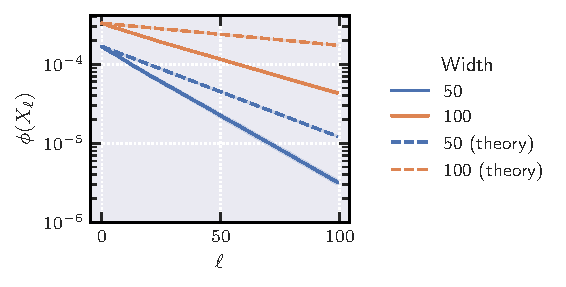
\includegraphics[width=0.7\textwidth]{figures/intro_figure_isogap.pdf}
    \caption{Isometry gap (y-axis, log-scale) in depth for an MLP with orthogonal weights, over randomly generated data. As predicted by Theorem~\ref{grad:thm:iso_gap_decay_in_depth}, isometry gap of representations vanishes at an exponential rate. The solid traces are averaged over $10$ independent runs, and the dashed traces show the theoretical prediction from Theorem~\ref{grad:thm:iso_gap_decay_in_depth}.}
    \label{grad:fig:linear_contrast} 
\end{figure}

\paragraph{Geometric interpretation of isometry.}
While the formula for isometry gap may seem enigmatic at first, it has a simple geometric interpretation that makes it intuitively understandable. The determinant $\det(X^\top X) = \det(X)^2$ is the squared volume of the parallelepiped spanned by the columns of $X$, while $\tr(X^\top X)$ is the sum squared-norms of the columns of $X$. Thus, the ratio between the two provides a scale-invariant notion of volume and isometry. On the one hand, if there is any collinearity between the columns, the volume will vanish and the isometry gap will be infinity, $\psi(X) = \infty$. On the other hand, $\psi(X) = 0$ implies $X^\top X$ is a scaled identity matrix. We will prove $\psi$ serves as a Lyapunov function for the chain of hidden representations $\{X_\ell\}_{\ell=0}^\infty$.

\paragraph{Theory for orthogonalization.}
The following theorem establishes the link between orthogonality of representations and depth. 
\begin{theorem}
\label{grad:thm:iso_gap_decay_in_depth}
There is an absolute constant $C$ such that for any layer $\ell \leq L$ we have
\begin{align}
    &\E \IG(X_{\ell+1})\le \IG(X_0)e^{-\ell/k}, & \text{where}&& k:=Cd^2(1+ d\IG(X_0))~.
\end{align}
\end{theorem}



Theorem~\ref{grad:thm:iso_gap_decay_in_depth} states that if the samples in the input batch are not linearly dependent, representations approach orthogonality at an exponential rate in depth. The orthogonalization in depth ensures the avoidance of the rank collapse of representations, which is a known barrier to training deep neural networks~\cite{daneshmand2020batch,saxe2013exact,bjorck2018understanding}. 

Figure~\ref{grad:fig:linear_contrast}
compares the established theoretical decay rate of $\psi$ with the practical rate. Interestingly, the plot confirms that the rate depends on width in practice, akin to the theoretical rate in Theorem~\ref{grad:thm:iso_gap_decay_in_depth}. It is worth mentioning that the condition on the input samples to not be linearly dependent is necessary to establish this result. One can readily check that starting from a rank-deficient input, neither matrix products, nor batch-normalization operations can increase the rank of the representations. Since this assumption is quantitative, we can numerically verify it by randomly drawing many input mini-batches and check if they are linearly dependent. For CIFAR10, CIFAR100, MNIST and FashionMNIST, we empirically tested that most batches across various batch sizes are full-rank (see Section~\ref{grad:sec:datasets_independence} for details on the average rank of a batch in these datasets). 

Theorem~\ref{grad:thm:iso_gap_decay_in_depth} distinguishes itself from the existing orthogonalization results in the literature~\citep{yang2018a,joudaki2023impact} as it is non-asymptotic and holds for networks with finite width. Since practical networks have finite width and depth, non-asymptotic results are crucial for their applicability to real-world settings. While \citet{daneshmand2021batch} provide a non-asymptotic bound for orthogonalization, the main result relies on an assumption that is hard to verify. 


\textit{Proof idea of Theorem~\ref{grad:thm:iso_gap_decay_in_depth}.}
We leverage a recent result established by  \citet{joudaki2023impact}, proving that the isometry gap does not decrease with BN layers. 
For all non-degenerate matrices $X \in \R^{d \times d}$, the following holds
    \begin{align*}
        \I(\BN(X))\geq \left(1+ \frac{\mathrm{variance}\{\|X_{j\cdot}\|\}_{j=1}^d}{(\mathrm{mean} \{\|X_{j\cdot}\|\}_{j=1}^d)^2}\right) \I(X)~.
    \end{align*}
Using the above result, we can prove that matrix multiplication with orthogonal weights also does not decrease isometry as stated in the next lemma. 
\begin{lemma}[Isometry after rotation]
\label{grad:lem:iso_rotation}
Let $X \in \R^{d\times d}$ and $W \in \R^{d\times d}$ be an orthogonal matrix and $X' = W X$; then,  
\begin{align}
   \I(\BN(X'))\geq \left(1+ \frac{\mathrm{variance}\{\|X'_{j\cdot}\|\}_{j=1}^d}{(\mathrm{mean} \{\|X'_{j\cdot}\|\}_{j=1}^d)^2}\right) \I(X)~.
\end{align}
\end{lemma}
%
It is straightforward to check that there exists at least an orthogonal matrix $W$ for which $\I(\BN(WX))=1$ (see Corollary~\ref{grad:cor:isometry_increase}). Thus, $\I(\cdot)$ strictly increases for some weight matrices, as long as $X$ is not orthogonal. When the distribution of $W$ is the Haar measure over the orthogonal group, we can leverage recent developments in Weingarten calculus~\citep{weingarten1978asymptotic, banica2011polynomial,collins2006integration,collins2022weingarten} to calculate a rate for the isometry increase in expectation: 
\begin{theorem}
    \label{grad:thm:iso_bound}
    Suppose $W \sim \mathbb{O}_d$ is a matrix drawn from $\mathbb{O}_d$ such that the distribution of $W$ and $UW$ are the same for all orthogonal matrices $U$. Let $\{\lambda_i\}_{i=1}^d$ be the eigenvalues of $XX^\top$. Then,
    % \begin{align}
    %     \E_W \left[\I(\BN(WX))\right ] \geq \left( \frac{1}{ 1 - \frac{\sum_{k=1}^d (\lambda_k - 1)^2}{2d^2(d+2)} } \right) \I(X)   
    % \end{align}
    \begin{align}
        \E_W \left[\I(\BN(WX))\right ] \geq \left( 1 - \frac{\sum_{k=1}^d (\lambda_k - 1)^2}{2d^2(d+2)} \right)^{-1} \I(X)   
    \end{align}
    holds for all $X = \BN(\cdot)$, with equality for orthogonal matrices.
\end{theorem}
The structure in $X$ induced by \BN{} ensures its eigenvalues lie in the interval $(0,1]$, in that the multiplicative factor in the above inequality is always greater than one. In other words, $\I(\cdot)$ increases by a constant factor in expectation that depends on how close $X$ is to an orthogonal matrix. 

The connection between Theorem~\ref{grad:thm:iso_bound} and the main isometry gap bound stated in Theorem~\ref{grad:thm:iso_gap_decay_in_depth} is established in the following Corollary (recall $\psi = -\log \I$). 

\begin{corollary}[Isometry gap bound]
% \label{grad:cor:isogap_bound}
Suppose the same setup as in Theorem~\ref{grad:thm:iso_bound}, where $X' = WX$. Then, we have:
\begin{align}
    \E_W[\IG(X') | X] \leq \IG(X) + \log \left(1 - \frac{\sum_k(\lambda_k - 1)^2}{2d^2(d+2)}\right).
\end{align}

  

\end{corollary}
  Notice that the term $\frac{\sum_{k=1}^d (\lambda_k - 1)^2}{2d^2(d+2)} = \mathcal{O}(\frac{1}{d})$, yielding $\log\left[1 - \frac{\sum_{k=1}^d (\lambda_k - 1)^2}{2d^2(d+2)} \right] \leq 0$.

% Finally, we establish the connection between the isometry bound and the isometry gap bound stated in Theorem~\ref{grad:thm:iso_gap_decay_in_depth} in Corollary~\ref{grad:cor:isogap_bound}. 
The rest of proof is based on an induction over the layers, presented in Appendices~\ref{grad:sec:conditional_orthonality} and~\ref{grad:sec:proof_isometry_depth}.  
% \end{itemize}
% \end{proof}

\subsection{Orthogonalization and gradient explosion}
There is a subtle connection between orthogonalization and gradient explosion. Suppose the input batch is rank-deficient, i.e., degenerate. As elaborated above, since all operations in our MLP can be formulated as matrix products, they cannot recover the rank of the representations, which thus remain degenerate. By perturbing the input such that it becomes full-rank, the output matrix becomes orthogonal, hence non-degenerate at an exponential rate in depth as proven in Theorem~\ref{grad:thm:iso_gap_decay_in_depth}. 

\begin{figure}[ht]
    \centering
    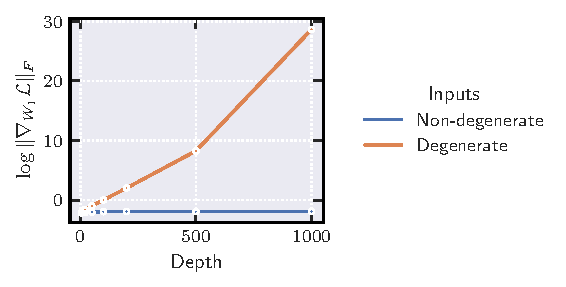
\includegraphics[width=0.7\textwidth]{figures/log_degenerate_inputs.pdf}
    \caption{Logarithmic plot for the gradient norm of the first layer for networks with different number of layers evaluated on degenerate (orange) and non-degenerate (blue) inputs. The degenerate inputs contain repeated samples from CIFAR10 in the batch, measured at initialization for MLPs of various depths. While gradients explode for degenerate inputs, there is no explosion for non-degenerate inputs. Traces are averaged over $10$ independent runs.}
    \label{grad:fig:degenerate_input}
\end{figure}
Thus, a slight change in inputs leads to a significant change in outputs from degeneracy to orthogonality. Considering that the gradient measures changes in the loss for infinitesimal inputs changes, the large changes in outputs potentially lead to gradient explosion. While this is only an intuitive argument, we observe that in practice the gradient does explode for degenerate inputs, as shown in Figure~\ref{grad:fig:degenerate_input}. 

Nonetheless, in Figure~\ref{grad:fig:degenerate_input} we observe that for non-degenerate inputs the gradient norm does not explode. In fact, we observe that inputs are often non-degenerate in practice (see Table~\ref{grad:tab:batch_degen} for details). Thus, an important question is whether the gradient norm remains bounded for non-degenerate input batches. Remarkably, we can not empirically verify that for \emph{all degenerate inputs} the gradient norm remains bounded. Therefore, a theoretical guarantee is necessary to ensure avoiding gradient explosion. 

% However, in Figure~\ref{grad:fig:degenerate_input},  we observe that for non-degenerate inputs the gradient norm does not explode. Since we observed that inputs often are non-degenerate in practice \alex{(see Table~\ref{grad:tab:batch_degen} for more details)} \hadi{reference?},  it is important to analyze the gradient norm for non-degenerate matrix. Notably, we can not empirically check the gradient norm explosion for all non-degenerate input matrices. Indeed, theory is a \emph{necessity} here but not a choice. Gradient explosion for a single non-degenerate input would cause numerical issues in training.  This motivates our theoretical analysis for gradient norm in the next section. 
% \begin{figure}[ht]
%     \centering
%     \includegraphics[width=0.6\linewidth]{figures/plots/degenerate_inputs.pdf}
%     \caption{Gradient explosion in depth for degenerate (orange) and non-degenerate (blue) inputs, where the degenerate inputs contain repeated samples in the batch, measured at initialization for MLPs of various depths. Degenerate inputs explode at an exponential rate in depth. Curves are averaged over $10$ independent runs, with the shaded region showing the $95\%$ confidence interval %\hadi{remove 20\% plot. Replace Gaussian with non-degenerate inputs and blue with degenerate inputs. Remove titles of 80\% on top. Replace initialization in the legend with inputs. We can also move it to the appendix}.\amir{Agreed.}}
%     }
%     \label{grad:fig:degenerate_input}
% \end{figure}



\subsection{Avoiding gradient explosion in depth}
\label{grad:sec:explosion}
So far, we have proven that the constructed network maintains the orthogonalization property of BN. Now, we turn our focus to the gradient analysis. The next theorem proves that the constructed network does not suffer from gradient explosion in depth for non-degenerate input matrices. 

\begin{theorem}\label{grad:thm:no_explosion}
Let the loss function $\Loss: \R^{d \times d} \to \R$ be $\mathcal{O}(1)$-Lipschitz, and input batch $X_0$ be non-degenerate. Then, there exists an absolute constant $C$ such that for all $\ell \leq L$ it holds
% \begin{align}
%     \E \left[ \log \| \nabla_{W_\ell} \mathcal{L}(X_\ell)\|\right] \le C d^5 \psi(X_0) \left(1 - e^{-L/k}\right), && k = C d^3(1+d\psi(X_0))
% \end{align}
\begin{align}
    \E \left[ \log \| \nabla_{W_\ell} \mathcal{L}(X_\ell)\|\right] \leq  Cd^5 (\psi(X_0)^3 + 1)
\end{align}

% \hadi{Is it possible to put theorem in one column. This is our main result and need more space. Figure 2 should be in section 3.2 somehow}
% \alex{yes, I'll reorder and fix spacing once we converge on the language and what versions of lemmas we leave in the main body} 
% \begin{align*}\tag{small isogap}
%     \E \left[ \log \| \nabla_{W_\ell} \mathcal{L}(X_\ell)\|\right] \le C d^4\psi(X_0)  \left(1 - e^{-\frac{L}{C d^4}}\right), 
% \end{align*}
% \begin{align*}\tag{big isogap}
%     \E \left[ \log \| \nabla_{W_\ell} \mathcal{L}(X_\ell)\|\right] \le C d^5\psi(X_0)^2  \left(1 - e^{-\frac{L}{C d^4}}\right), 
% \end{align*}
where the expectation is over the random orthogonal weight matrices. 
\end{theorem}
% \begin{remark}
%     Note that while the right-hand side of the Theorem~\ref{grad:thm:no_explosion} increases with depth $L$, as the depth increases, it stabilises around a finite value. Thus, even in the limit of infinite depth we have $\E \left[ \log \| \nabla_{W_\ell} \mathcal{L}(X_\ell)\|\right] \le C d^5 (\psi(X_0)^3 + 1).$
% \end{remark}
\begin{remark}
    For degenerate inputs $\psi(X_0) = \infty$ holds, in that the bound becomes vacuous.  
\end{remark}
\begin{remark}
    The $\mathcal{O}(1)$-Lipschitz condition holds in many practical settings. For example, in a classification setting, MSE and cross entropy losses obey the $\mathcal{O}(1)$-Lipschitz condition (see Lemma~\ref{grad:lem:lipschitz}).
    % \hadi{I am not sure about this. how we can prove this? }
\end{remark}

\begin{figure}[ht]
    \centering
    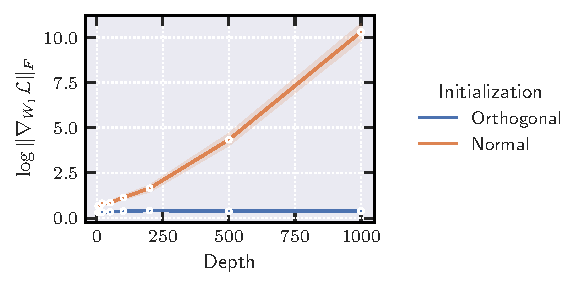
\includegraphics[width=0.75\textwidth]{figures/log_intro_figure_grad.pdf}
    \caption{Logarithmic plot for the gradient norm of the first layer for networks with different number of layers evaluated on CIFAR10. For Gaussian weights (orange) the gradient-norm grows at an exponential rate, as predicted by \citet[Theorem 3.9]{yang2018a}, while for orthogonal weights (blue) gradients remain bounded by a constant, validating Theorem~\ref{grad:thm:no_explosion}. Traces are averaged over $10$ runs and shaded regions denote the $95\%$ confidence intervals.}
    \label{grad:fig:linear_contrast_grad} 
\end{figure}

% Figure~\ref{grad:fig:linear_contrast_grad} shows that log-norms of the gradients do not explode in depth, thus validating Theorem~\ref{grad:thm:no_explosion}. In contrast, we observe in this figure that when using Gaussian weights, the gradients grow exponentially in depth, which is consistent with \citet[Theorem 3.9]{yang2018a}. 

Note that the bound is stated for the expected value of log-norm of the gradients, which can be interpreted as bits of precision needed to store the gradient matrices. Thus, the fact that depth does not appear in any form in the upper bound of Theorem~\ref{grad:thm:no_explosion} points out that training arbitrarily deep MLPs with orthogonal weights will not face numerical issues that arise with Gaussian weights~\cite{yang2018a} as long as the inputs are non-degenerate. Such guarantees are necessary to ensure backpropagation will not face numerical issues.  

 Theorem~\ref{grad:thm:no_explosion} states that as long as the input samples are not linearly dependent, the gradients remain bounded for any arbitrary depth $L$. As discussed in the previous section and evidenced in Figure~\ref{grad:fig:degenerate_input}, this is necessary to avoid gradient explosion. Therefore, the upper bound provided in Theorem~\ref{grad:thm:no_explosion} is tight in terms of inputs constraints. Furthermore, as mentioned before, random batches sampled from commonly used benchmarks, such as CIFAR10, CIFAR100, MNIST, and FashionMNIST, are non-degenerate in most practical cases (see Section~\ref{grad:sec:datasets_independence} for more details). Thus, the assumptions and thereby assertions of the theorem are valid for all practical purposes.

To the best of our knowledge, Theorem~\ref{grad:thm:no_explosion} is the first non-asymptotic gradient analysis that holds for networks with batch normalization and finite width. Previous results heavily rely on mean field analyses in asymptotic regimes, where the network width tends to infinity~\citep{yang2018a}. While mean field analyses have brought many insights about the rate of gradient explosion, they are often specific to Gaussian weights. Here, we show that non-Gaussian weights can avoid gradient explosion, which has previously been considered ``unavoidable''~\citep{yang2018a}. Figure~\ref{grad:fig:linear_contrast_grad} illustrates this pronounced discrepancy.  

\textit{Proof idea of Theorem~\ref{grad:thm:no_explosion}.}
    The first important observation is that, due to the chain rule, we can bound the log-norm of the gradient of a composition of functions, by bounding the summation of the log-norms of the input-output Jacobian of each layer, plus two additional terms corresponding to the loss term and the gradient of the first layer in the chain. If we discount the effect of the first and last terms, the bulk of the analysis is dedicated to bounding the total sum of log-norms of per layer input-output Jacobian, i.e., the fully connected and batch normalization layers. The second observation is that because the weights are only rotations, their Jacobian has eigenvalues equal to $1.$ Thus, the log-norm of gradients corresponding to fully connected layers vanish. What remains is to show that for any arbitrary depth $\ell,$ the log-norm of gradients of batch normalization layers also remains bounded. The main technical novelty for proving this step is showing that the log-norm of the gradient of $\BN$ layers is upper bounded by the isometry gap of pre-normalization matrices. Thus, we can invoke the exponential decay in isometry gap stated in Theorem~\ref{grad:thm:iso_gap_decay_in_depth} to establish a bound on the log-norm of the gradient of these layers. Finally, since the decay in isometry gap is exponentially fast, the bound on the total sum of log-norm of the gradients amounts to a geometric sum that remains bounded for any arbitrary depth $\ell.$ 


    


\section{Implications on training}
\label{grad:sec:experiments}
In this section, we experimentally validate the benefits of avoiding gradient explosion and rank collapse for training.
Thus far, we have proved that our constructed neural network with BN does not suffer from gradient explosion in Theorem~\ref{grad:thm:no_explosion}, and does not have the rank collapse issue in depth via the orthogonalization property established in Theorem~\ref{grad:thm:iso_gap_decay_in_depth}. We find that the constructed MLP is therefore less prone to numerical issues that arise when training deep networks. %Since our MLP construction simultaneously avoids exploding gradients and rank collapse, it is less prone to numerical issues that arise when training deep networks. 


\begin{figure}[ht]
    \centering
 \includegraphics[width=1\linewidth]{figures/train_CIFAR10.pdf}
 \vspace{-.8cm}
    \caption{Contrasting the training accuracy of MLPs with BN and shaped sin, shaped tanh and identity activations, on the CIFAR10 dataset. The identity activation performs much worse than the nonlinearities, confirming that the $\sin$ and $\tanh$ networks are not operating in the linear regime. The networks are trained with vanilla SGD and the hyperparameters are width $100$, batch size $100$, learning rate $0.001$.}
    \vspace{-0.3cm}
    \label{grad:fig:train_cifar10}
\end{figure}


By avoiding gradient explosion and rank collapse in depth, we observe that the optimization with vanilla minibatch Stochastic Gradient Descent (SGD) exhibits an almost depth-independent convergence rate for linear MLPs. In other words, the number of iterations to get to a certain accuracy does not vary widely between networks with different depths. Figure~\ref{grad:fig:train_cifar10} (c) shows the convergence of SGD for CIFAR10, with learning rate $0.001$, for MLPs with width $d=100$ and batch size $n=100.$ While the SGD trajectory strongly diverges from the initial conditions that we analyze theoretically, Figure~\ref{grad:fig:train_cifar10} shows that the gradients remain stable during training, as well as the fact that different depths exhibit largely similar accuracy curves. 




While the empirical evidence for our MLP with linear activation is encouraging, non-linear activations are essential parts of feature learning~\cite{nair2010rectified,klambauer2017self,hendrycks2016gaussian,maas2013rectifier}. However, introducing non-linearity violates one of the key parts of our theory, in that it prevents representations from reaching perfect isometry (see Figure~\ref{grad:fig:nonlinear_contrast} for details on the connection between non-linearities and gradient explosion in depth). Intuitively, this is due to the fact that non-linear layers, as opposed to rotations and batch normalization, perturb the isometry of representations and prevent them from reaching zero isometry gap in depth. This problem turns out to be not just a theoretical nuisance, but to play a direct role in the gradient explosion behavior.
% Figure~\ref{grad:fig:nonlinear_contrast} shows the gradient norms  explode at a fixed multiplicative rate after the isometry gap stabilizes. This means that the MLPs with non-linear activations are not able to avoid gradient explosion, in contrast to the linear case. 
While the situation may seem futile at first, it turns out that activation shaping~\citep{li2022neural,zhang2022deep,martens2021rapid,he2023deep,noci2023shaped} can alleviate this problem, which is discussed next. For the remainder of this section, we focus on the training of MLPs with non-linear activations, as well as standard batch normalization and fully connected layers.

\section{Activation shaping based on the theoretical analysis} 
In recent years, several works have attempted to overcome the challenges of training very deep networks by parameterizing activation functions. 
In a seminal work, ~\citet{martens2021rapid} propose \textit{deep kernel shaping}, which is aimed at facilitating the training of deep networks without relying on skip connections or normalization layers, and was later extended to LeakyReLU in \textit{tailored activation transformations}~\citep{zhang2022deep}. In a similar direction, ~\citet{li2022neural} propose \textit{activation shaping} in order to avoid a degenerate output covariance. While the mechanism proposed by~\citet{li2022neural} covers both smooth and non-smooth activations, we focus on their result for LeakyReLU, which consists of shaping the negative slope of the activation towards identity to ensure that the output covariance matrix remains non-degenerate when the networks becomes very deep. 

Since kernel and activation shaping aim to replace normalization, they have not been used in conjunction with normalization layers. 
In fact, in networks with batch normalization, even linear activations have non-degenerate outputs~\citep{daneshmand2021batch,yang2018a} and exploding gradients~\citep{yang2018a}. Thus, shaping activations towards identity in the presence of normalization layers may seem fruitless. Remarkably, we empirically demonstrate that we can leverage activation shaping to avoid gradient explosion in depth by using a pre-activation gain at each layer. 

% \citet{yang2018a} conclude that in the presence of batch normalization, linear activations suffer from the smallest rate of gradient explosion. However, even linear activations exhibit exponential gradient explosion in the number of layers. In comparison, our activation shaping scheme achieves a constant gradient norm in depth. This contrast can be attributed to using orthogonal weight matrices, as well as a careful activation shaping mechanism. 

\begin{figure}[ht] 
  \centering
  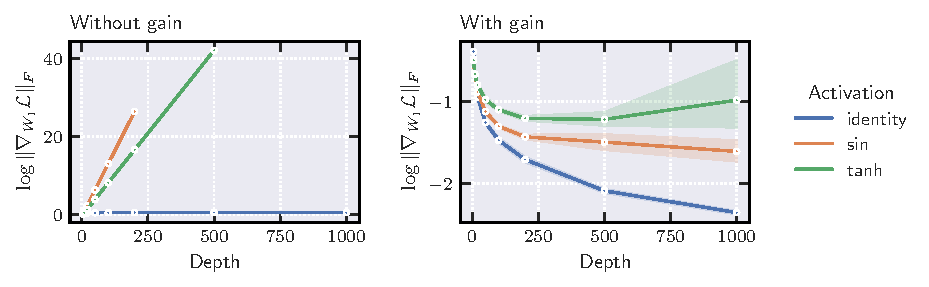
\includegraphics[width=0.8\linewidth]{figures/log_gain_vs_no_gain.pdf}
  \vspace{-.2cm}
  \caption{Logarithmic plot contrasting the effect of gain on the gradient at initialization of the first layer, for networks with different number of layers initialized with orthogonal weights, BN and different activations, evaluated on CIFAR10. The networks have hyperparameters width $100$, batch size $100$. Traces are averaged over $10$ independent runs, with the shades showing the $95\%$ confidence interval.}
  \label{grad:fig:gain_effect}
\end{figure}
Inspired by our theory, we develop a novel activation shaping scheme for networks with BN. The main strategy consists of shaping the activation function towards a linear function across the layers. Our activation shaping consists of tuning the gain of the activation, i.e., tuning $\alpha$ for $\sigma(\alpha x).$ We consider non-linear activations $\sigma \in \{\tanh, \sin\}.$  


The special property that both $\tanh$ and $\sin$ activations have in common is that they are centered, $\act(0)=0,$ are differentiable around the origin $\act'(0)=1,$ and have bounded gradients $\act'(x) \leq 1, \forall x$. Therefore, by tuning the per-layer pre-activation gain $\alpha_\ell$ towards $0$, the non-linearities behave akin to the identity function. This observation inspires us to study the relationship between the rate of gradient explosion for each layer as a function of the gain parameter $\alpha_\ell$. Formally, we consider an MLP with shaped activations using gain $\alpha_\ell$ for the $\ell$th layer, that has the update rule
\begin{align}
    X_{\ell + 1} = \act(\alpha_\ell \BN(W_\ell X_\ell))~.
    \label{grad:eqn:mlp_nonlinear}
\end{align}

% \begin{figure}[t]
%     \centering
%  \includegraphics[width=1\linewidth]{figures/plots/accuracy_plots/train_CIFAR10.pdf}
%  \vspace{-.8cm}
%     \caption{Contrasting the training accuracy of MLPs with BN and shaped sin, tanh, and identity activations on CIFAR10. The identity activation performs much worse than the nonlinearities, indicating the fact that the sin and tanh networks are not operating in the linear regime. The networks are trained with vanilla SGD and the hyperparameters are width $100$, batch size $100$, learning rate $0.001$.}
%     \label{grad:fig:train_cifar10}
% \end{figure}



Since the gradient norm has an exponential growth in depth, as shown in Figure~\ref{grad:fig:gain_effect}, we can compute the slope of the linear growth rate of log-norm of gradients in depth. We define the rate of explosion for a model of depth $L$ and gain $\alpha_\ell$ at layer $\ell$ as the slope of the log norm of the gradients $R(\ell, \alpha_\ell)$. We show in Figure~\ref{grad:fig:gain_effect} that by tuning the gain properly, we are able to reduce the exponential rate of the log-norm of the gradients by diminishing the slope of the rate curve and achieve networks trainable at arbitrary depths, while still maintaining the benefits of the non-linear activation. The main idea for our activation shaping strategy is to have a bounded total sum of rates across layers, by ensuring faster decay than a harmonic series (see App.~\ref{grad:sec:shaping} for more details on activation shaping). Figure~\ref{grad:fig:gain_effect} illustrates that this activation shaping strategy effectively avoids gradient explosion while maintaining the signal propagation and orthogonality of the outputs in depth. Furthermore, Figure~\ref{grad:fig:train_cifar10} shows that the training accuracy remains largely depth-independent. For further experiments using activation shaping, see Section~\ref{grad:sec:other_experiments}.



\section{Discussion}


\paragraph{Implicit bias of SGD towards orthogonality in optimization.} 
\begin{figure}[ht]
    \centering
    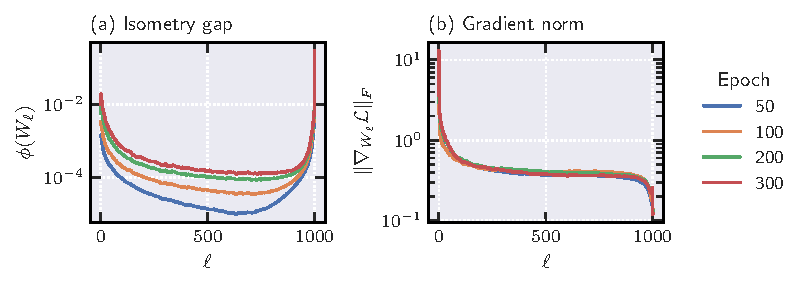
\includegraphics[width=0.9\linewidth]{figures/weight_grads_during_training_1000.pdf}
    \vspace{-.5cm}
    \caption{\textbf{Implicit orthogonality bias of SGD.} Training an MLP with width $d=100,$ batch size $n=100,$ and depth $L=1000,$ activation $\tanh$, using SGD with $\text{lr}=0.001$ (a) Isometry gap (y-axis; log-scale) of weight matrices across all layers throughout training. (b) Gradient norms at each layer during training. }
    \label{grad:fig:ortho_during_training_1000}    
\end{figure}
Optimization over orthogonal matrices has been an effective approach for training deep neural networks. Enforcing orthogonality during training ensures that the spectrum of the weight matrices remains bounded, which prevents gradient vanishing and explosion in depth. \citet{vorontsov2017orthogonality} study how different orthogonality constraints affect training performance in RNNs. For example \citet{lezcano2019cheap} leverage the exponential map on the orthogonal group, \citet{jose2018kronecker} decompose RNN transition matrices in Kronecker factors and impose soft constraints on each factor and \citet{mhammedi2017efficient} introduce a constraint based on Householder matrices.


While these studies \emph{enforce} orthogonality constraints, one of our most striking empirical observations is that when our MLP grows very deep, the middle layers remain almost orthogonal even after many steps of SGD. As shown in Figure~\ref{grad:fig:ortho_during_training_1000}, for $1000$ layer networks, the middle layers remain orthogonal during training. One could hypothesize that this is due to small gradients in these layers. In Figure~\ref{grad:fig:ortho_during_training_1000}, we observe that the gradients of these middle layers are not negligible. Thus, in our MLP construction, both with linear activation and with activation shaping, the gradient dynamics have an \emph{implicit bias} to optimize over the space of orthogonal matrices. The mechanisms underlying this implicit orthogonality bias will be an ample direction for future research.



